% Vietnamese translation for OI Public Library
% Source-PDF: IOI中国国家候选队论文/2007/day1/3.仇荣琦《欧拉回路性质与应用探究》.pdf
\documentclass[11pt]{article}
\usepackage{tikz}
\usetikzlibrary{arrows.meta,calc,positioning}
\usepackage{oipl-vn}

\newcommand{\Oh}{\mathcal{O}}
\newcommand{\indeg}{\operatorname{in}}
\newcommand{\outdeg}{\operatorname{out}}
\newcommand{\dist}{\operatorname{dist}}

\title{Khảo sát tính chất và ứng dụng của chu trình Euler}
\author{Qiu Rongqi\\Trung học trực thuộc Đại học Sư phạm Hồ Nam}
\date{}

\begin{document}
\maketitle

\origtitle{Properties and applications of Euler circuits}
\sourcepath{IOI China candidate team papers / 2007 / day 1 / Qiu Rongqi}

\begin{abstract}
Chu trình Euler, còn gọi là bài toán ``vẽ một nét'', là một dạng bài toán về
khả năng đi qua trong lý thuyết đồ thị. Bài viết trước hết giới thiệu các
kiến thức lý thuyết liên quan tới chu trình Euler và thuật toán tìm chu trình
Euler. Sau đó, thông qua một số ví dụ, bài viết trình bày vài lớp bài toán
điển hình gắn với chu trình Euler. Cuối cùng, bài viết tổng kết mô hình chu
trình Euler, chỉ ra đặc điểm và ưu thế của nó.
\end{abstract}

\paragraph{Từ khóa.}
Chu trình Euler; đường đi Euler.

\tableofcontents

\section{Dẫn nhập}

Bài toán chu trình Euler là một trong những bài toán cổ nhất của lý thuyết đồ
thị. Nó ra đời tại thành phố cổ Konigsberg ở châu Âu thế kỷ XVIII. Sông
Pregel chảy qua thành phố này; giữa hai bờ sông và hai hòn đảo ở giữa sông,
người ta xây bảy cây cầu.

\begin{center}
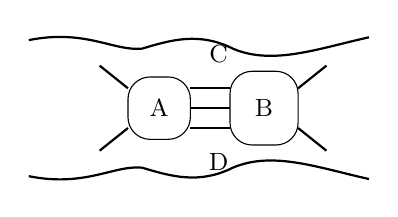
\begin{tikzpicture}[scale=0.72, every node/.style={font=\small}]
  \draw[thick] (-3,1.2) .. controls (-2,1.4) and (-1.5,1.0) .. (-1.0,1.05)
    .. controls (-0.5,1.2) and (0.0,1.35) .. (0.6,1.05)
    .. controls (1.3,0.75) and (2.1,1.05) .. (3,1.25);
  \draw[thick] (-3,-1.2) .. controls (-2,-1.4) and (-1.5,-1.0) .. (-1.0,-1.05)
    .. controls (-0.5,-1.2) and (0.0,-1.35) .. (0.6,-1.05)
    .. controls (1.3,-0.75) and (2.1,-1.05) .. (3,-1.25);
  \draw[rounded corners=8pt] (-1.25,0.55) rectangle (-0.15,-0.55);
  \draw[rounded corners=8pt] (0.55,0.65) rectangle (1.75,-0.65);
  \node at (-0.7,0) {A};
  \node at (1.15,0) {B};
  \node at (0.35,0.95) {C};
  \node at (0.35,-0.95) {D};
  \foreach \y in {-0.35,0,0.35} \draw[thick] (-0.15,\y) -- (0.55,\y);
  \draw[thick] (-1.25,0.35) -- (-1.75,0.75);
  \draw[thick] (-1.25,-0.35) -- (-1.75,-0.75);
  \draw[thick] (1.75,0.35) -- (2.25,0.75);
  \draw[thick] (1.75,-0.35) -- (2.25,-0.75);
\end{tikzpicture}\\
\small Hình 1: sơ đồ bảy cây cầu Konigsberg.
\end{center}

Người dân thường đi dạo ở đây, rồi nảy sinh câu hỏi: có thể tìm một cách đi
sao cho xuất phát từ nhà, đi qua mỗi cây cầu đúng một lần, rồi quay lại nhà
hay không? Viết bằng ngôn ngữ toán học, đó là bài toán tìm một chu trình trong
đồ thị sao cho nó đi qua mỗi cạnh đúng một lần. Đây chính là bài toán bảy cây
cầu Konigsberg nổi tiếng.

\begin{center}
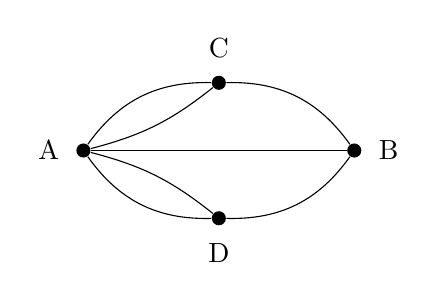
\begin{tikzpicture}[scale=0.86, every node/.style={circle,fill=black,inner sep=1.8pt,label distance=2pt}]
  \node[label=left:{A}] (A) at (-2,0) {};
  \node[label=right:{B}] (B) at (2,0) {};
  \node[label=above:{C}] (C) at (0,1.0) {};
  \node[label=below:{D}] (D) at (0,-1.0) {};
  \draw (A) -- (B);
  \draw (A) to[bend left=28] (C);
  \draw (C) to[bend left=28] (B);
  \draw (A) to[bend right=28] (D);
  \draw (D) to[bend right=28] (B);
  \draw (A) to[bend left=12] (D);
  \draw (A) to[bend right=12] (C);
\end{tikzpicture}\\
\small Hình 2: mô hình đồ thị của bài toán bảy cây cầu.
\end{center}

Rất nhiều người say mê bài toán này đã thử giải nhưng đều thất bại. Khi bài
toán đến tay Leonhard Euler (1707--1783), nó lập tức thu hút sự chú ý của nhà
toán học lớn này. Sau khi nghiên cứu kỹ, năm 1736 Euler công bố bài báo về
bảy cây cầu Konigsberg: ông không chỉ chứng minh thành công rằng bài toán bảy
cây cầu vô nghiệm, mà còn tìm được điều kiện cần và đủ để một đồ thị tổng quát
có loại chu trình này. Để tưởng nhớ Euler, hậu thế gọi các chu trình như vậy
là chu trình Euler.

Chu trình Euler có ứng dụng rộng trong thi tin học. Những năm gần đây, nhiều
bài thi thuộc các loại khác nhau đã xuất hiện dưới dạng liên quan tới nó. Bài
viết này giới thiệu kiến thức cơ bản về chu trình Euler và phân tích ứng dụng
thực tế của nó qua một vài bài mẫu.

\section{Kiến thức liên quan}

Trước hết ta giới thiệu các khái niệm và định lý cần dùng. Giả sử
\(G=(V,E)\) là một đồ thị.

\paragraph{Chu trình Euler.}
Một chu trình trong \(G\) đi qua mỗi cạnh một lần và chỉ một lần được gọi là
chu trình Euler.

\paragraph{Đường đi Euler.}
Một đường đi trong \(G\) đi qua mỗi cạnh một lần và chỉ một lần được gọi là
đường đi Euler.

\paragraph{Đồ thị Euler.}
Đồ thị có chu trình Euler được gọi là đồ thị Euler.

\paragraph{Đồ thị nửa Euler.}
Đồ thị có đường đi Euler nhưng không có chu trình Euler được gọi là đồ thị nửa
Euler.

Trong các thảo luận sau, ta giả sử \(G\) không có đỉnh cô lập, tức đỉnh bậc
\(0\). Nếu có, trước hết xóa mọi đỉnh cô lập khỏi đồ thị. Rõ ràng thao tác này
không ảnh hưởng tới sự tồn tại của chu trình Euler trong \(G\).

Ta thường cần phán đoán một đồ thị có phải đồ thị Euler hoặc nửa Euler hay
không, đồng thời tìm một chu trình hoặc đường đi tương ứng. Với đồ thị vô
hướng, ta có kết luận sau.

\paragraph{Định lý 1.}
Đồ thị vô hướng \(G\) là đồ thị Euler khi và chỉ khi \(G\) liên thông và mọi
đỉnh đều có bậc chẵn.

\paragraph{Chứng minh.}
Chiều cần. Giả sử \(C\) là một chu trình Euler của \(G\). Vì \(C\) đi qua mọi
cạnh của \(G\), mà \(G\) không có đỉnh cô lập, nên \(C\) cũng đi qua mọi đỉnh
của \(G\). Do đó \(G\) liên thông. Với một đỉnh bất kỳ \(v\), mỗi lần \(C\) đi
qua \(v\), nó đi vào bằng một cạnh rồi đi ra bằng một cạnh khác; số cạnh kề
với \(v\) mà \(C\) sử dụng vì thế là chẵn. Do \(C\) đi qua mọi cạnh của \(G\)
đúng một lần, bậc của \(v\) là chẵn.

Chiều đủ. Giả sử \(G\) không chứa chu trình. Vì \(G\) liên thông, \(G\) phải là
một cây, nên \(|E|=|V|-1\). Mọi đỉnh của \(G\) đều có bậc chẵn và không có
đỉnh cô lập, nên mỗi đỉnh có bậc ít nhất \(2\). Theo định lý bắt tay,
\[
  |E|=\frac12\sum_{v\in V}d(v)\ge |V|,
\]
mâu thuẫn với \(|E|=|V|-1\). Vì vậy trong \(G\) tồn tại chu trình.

Chọn một chu trình đơn có số cạnh lớn nhất:
\[
  C=\{e_1=(v_0,v_1), e_2=(v_1,v_2),\ldots,
       e_m=(v_{m-1},v_0)\}.
\]
Ta chứng minh \(C\) là chu trình Euler của \(G\).

Giả sử \(C\) chưa phải chu trình Euler. Khi đó trên \(C\) tồn tại một đỉnh
\(v_k\) sao cho bậc của nó lớn hơn số cạnh kề với nó đã được \(C\) đi qua. Đặt
\(v'_0=v_k\). Từ \(v'_0\) có một cạnh \(e'_1=(v'_0,v'_1)\) không thuộc \(C\).
Nếu \(v'_1=v'_0\), cạnh này là một khuyên tại \(v'_0\), có thể ghép vào \(C\)
để được chu trình lớn hơn. Nếu \(v'_1\ne v'_0\), vì bậc của \(v'_1\) là chẵn
và số cạnh kề với \(v'_1\) xuất hiện trong \(C\) cũng là chẵn, chắc chắn tồn
tại một cạnh \(e'_2=(v'_1,v'_2)\) không thuộc \(C\). Tiếp tục như vậy, ta tìm
được các cạnh không thuộc \(C\)
\[
  e'_3=(v'_2,v'_3),\ldots,e'_k=(v'_{k-1},v'_0).
\]
Do đó \(C'=\{e'_1,e'_2,\ldots,e'_k\}\) là một chu trình mới. Ghép \(C'\) vào
\(C\) sẽ tạo ra một chu trình có nhiều cạnh hơn, mâu thuẫn với cách chọn \(C\).
Vì vậy \(C\) là chu trình Euler của \(G\).

\paragraph{Hệ quả 1.}
Đồ thị vô hướng \(G\) là đồ thị nửa Euler khi và chỉ khi \(G\) liên thông, đúng
hai đỉnh có bậc lẻ và mọi đỉnh còn lại có bậc chẵn.

\paragraph{Chứng minh.}
Chiều cần. Giả sử \(P\) là một đường đi Euler của \(G\):
\[
  P=\{e_1=(v_0,v_1), e_2=(v_1,v_2),\ldots,
       e_m=(v_{m-1},v_m)\}.
\]
Vì \(P\) đi qua mọi cạnh của \(G\), mà \(G\) không có đỉnh cô lập, nên \(P\)
cũng đi qua mọi đỉnh, do đó \(G\) liên thông. Tại \(v_0\), số lần \(P\) đi vào
ít hơn số lần đi ra \(1\); tại \(v_m\), số lần đi vào nhiều hơn số lần đi ra
\(1\). Vì vậy \(v_0\) và \(v_m\) có bậc lẻ. Với mọi đỉnh khác
\(v_k\ne v_0,v_m\), số lần đi vào bằng số lần đi ra, nên bậc của \(v_k\) là
chẵn.

Chiều đủ. Gọi \(v_1,v_2\) là hai đỉnh bậc lẻ duy nhất của \(G\). Thêm vào
\(G\) một cạnh ảo \(e_0=(v_1,v_2)\) để được \(G'\). Khi đó mọi đỉnh của \(G'\)
đều có bậc chẵn, nên \(G'\) có chu trình Euler \(C'\). Xóa \(e_0\) khỏi \(C'\)
ta thu được một đường đi từ \(v_1\) tới \(v_2\), chính là đường đi Euler của
\(G\).

Với đồ thị có hướng, ta có các kết luận tương tự. Ở đây, đồ thị nền của một đồ
thị có hướng là đồ thị vô hướng thu được sau khi bỏ qua hướng của mọi cạnh.

\paragraph{Định lý 2.}
Đồ thị có hướng \(G\) là đồ thị Euler khi và chỉ khi đồ thị nền của \(G\) liên
thông và với mọi đỉnh, bậc vào bằng bậc ra.

\paragraph{Hệ quả 2.}
Đồ thị có hướng \(G\) là đồ thị nửa Euler khi và chỉ khi đồ thị nền liên
thông, tồn tại một đỉnh \(u\) có bậc vào lớn hơn bậc ra \(1\), một đỉnh \(v\)
có bậc vào nhỏ hơn bậc ra \(1\), còn các đỉnh khác đều có bậc vào bằng bậc ra.

Hai kết luận trên được chứng minh tương tự định lý 1 và hệ quả 1.

Chứng minh của định lý 1 có tính xây dựng, nên có thể dùng để tìm chu trình
Euler. Dưới đây lấy đồ thị vô hướng làm ví dụ.

\paragraph{Tính chất 1.}
Giả sử \(C\) là một chu trình đơn trong đồ thị Euler \(G\). Xóa các cạnh của
\(C\) khỏi \(G\) để được \(G'\). Khi đó mỗi thành phần liên thông cực đại của
\(G'\) đều có chu trình Euler.

\paragraph{Chứng minh.}
Nếu \(G\) vô hướng, mọi đỉnh của \(G'\) vẫn có bậc chẵn. Nếu \(G\) có hướng,
mọi đỉnh của \(G'\) vẫn có bậc vào bằng bậc ra.

\paragraph{Tính chất 2.}
Giả sử \(C_1\) và \(C_2\) là hai chu trình đơn của \(G\), không có cạnh chung
nhưng có ít nhất một đỉnh chung. Khi đó ta có thể ghép chúng thành một chu
trình đơn mới \(C'\).

\paragraph{Chứng minh.}
Đi theo \(C_1\) tới một đỉnh chung, đi hết \(C_2\), rồi tiếp tục phần còn lại
của \(C_1\). Vì hai chu trình không có cạnh chung, cách ghép này đi qua mỗi
cạnh trong \(C_1\cup C_2\) đúng một lần.

\begin{center}
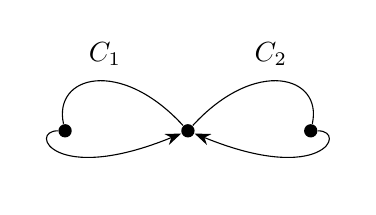
\begin{tikzpicture}[scale=0.78, every node/.style={circle,fill=black,inner sep=1.7pt}]
  \node (x) at (0,0) {};
  \node (l) at (-2.0,0) {};
  \node (r) at (2.0,0) {};
  \draw[-{Stealth[length=2mm]}] (x) .. controls (-1.1,1.2) and (-2.2,0.9) .. (l)
    .. controls (-2.6,0.0) and (-2.2,-0.9) .. (x);
  \draw[-{Stealth[length=2mm]}] (x) .. controls (1.1,1.2) and (2.2,0.9) .. (r)
    .. controls (2.6,0.0) and (2.2,-0.9) .. (x);
  \node[fill=none,draw=none] at (-1.35,1.25) {\(C_1\)};
  \node[fill=none,draw=none] at (1.35,1.25) {\(C_2\)};
\end{tikzpicture}\\
\small Hình 3: ghép hai chu trình có đỉnh chung.
\end{center}

Từ đó nhận được thuật toán tìm chu trình Euler của đồ thị Euler \(G\):
\begin{enumerate}
  \item Tìm tùy ý một chu trình \(C\) trong \(G\).
  \item Xóa các cạnh thuộc \(C\) khỏi \(G\).
  \item Trong từng thành phần liên thông cực đại của đồ thị còn lại, tìm một
  chu trình Euler.
  \item Ghép các chu trình Euler của các thành phần vào \(C\), thu được chu
  trình Euler của \(G\).
\end{enumerate}

Mã giả quen thuộc của thuật toán như sau.
\begin{verbatim}
procedure euler_circuit(start)
    for each neighbor v of start do
        if edge(start, v) is unused then
            mark edge(start, v)
            mark edge(v, start)        // remove this line for directed graphs
            euler_circuit(v)
            push edge(start, v) into stack S
        end if
    end for
end procedure
\end{verbatim}
Lấy lần lượt các cạnh ra khỏi ngăn xếp \(S\) sẽ nhận được chu trình Euler của
\(G\).

Trong quá trình chạy, mỗi cạnh được thăm nhiều nhất hai lần, nên độ phức tạp
thời gian là \(\Oh(|E|)\). Khi ứng dụng thực tế, cài đặt đệ quy có thể gây tràn
ngăn xếp vì độ sâu đệ quy tối đa đạt \(|E|\). Vì thế ta thường chuyển nó sang
dạng không đệ quy. Với đồ thị có hướng, ta vẫn dùng thuật toán trên, chỉ cần
bỏ dòng đánh dấu cạnh ngược.

Phần trên đã giới thiệu kiến thức và thuật toán liên quan tới chu trình Euler.
Trong bài toán thực tế, phần linh hoạt và thách thức hơn lại là lập mô hình.
Phần tiếp theo phân tích một số ví dụ để khảo sát cách xây dựng mô hình chu
trình Euler, qua đó giúp hiểu sâu hơn thuật toán này.

\section{Ví dụ}

\subsection{Ví dụ 1: Trò chơi ghép từ}

\paragraph{Mô tả bài toán.}
Có \(N\) tấm bảng, mỗi tấm ghi một từ tiếng Anh chỉ gồm chữ cái thường. Cần
sắp xếp các tấm bảng theo một thứ tự sao cho trong hai tấm kề nhau, chữ cái
cuối của từ trên tấm trước bằng chữ cái đầu của từ trên tấm sau. Hãy viết
chương trình phán đoán có thể đạt yêu cầu đó hay không; nếu có, hãy đưa ra một
thứ tự phù hợp.

Quy mô dữ liệu: \(1\le N\le 100000\).

\paragraph{Phân tích.}
Từ điều kiện đề bài, ta rất dễ nhận được mô hình trực quan sau.

\paragraph{Mô hình 1.}
Lấy \(N\) tấm bảng làm đỉnh. Nếu chữ cái cuối của tấm \(A\) bằng chữ cái đầu
của tấm \(B\), nối một cạnh có hướng từ \(A\) tới \(B\). Khi đó bài toán trở
thành tìm một đường đi đi qua mỗi đỉnh đúng một lần, tức đường Hamilton. Tuy
nhiên, tìm đường Hamilton là một bài toán rất khó; mô hình này không đem lại
lợi thế thuật toán nào.

\begin{center}
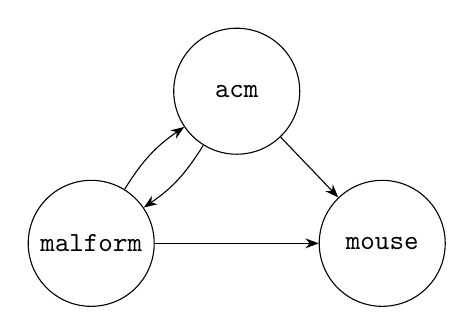
\begin{tikzpicture}[>=Stealth, scale=0.84,
  word/.style={circle,draw,minimum size=16mm,font=\ttfamily}]
  \node[word] (acm) at (0,1.7) {acm};
  \node[word] (mal) at (-2.2,-0.6) {malform};
  \node[word] (mouse) at (2.2,-0.6) {mouse};
  \draw[->] (acm) to[bend left=12] (mal);
  \draw[->] (mal) to[bend left=12] (acm);
  \draw[->] (acm) -- (mouse);
  \draw[->] (mal) -- (mouse);
\end{tikzpicture}\\
\small Hình 4: mô hình lấy từng từ làm đỉnh.
\end{center}

\paragraph{Mô hình 2.}
Điểm thất bại của mô hình 1 là thông tin cần duyệt, tức từng tấm bảng, lại
nằm trên đỉnh; trong khi bài toán duyệt đỉnh khó xử lý. Ta thử đưa thông tin
cần duyệt lên cạnh: lấy \(26\) chữ cái làm đỉnh; với mỗi tấm bảng, nếu chữ cái
đầu là \(c_1\), chữ cái cuối là \(c_2\), nối một cạnh có hướng từ \(c_1\) tới
\(c_2\). Các đỉnh không xuất hiện đều là đỉnh cô lập và có thể xóa trước. Khi
đó bài toán trở thành tìm một đường đi đi qua mỗi cạnh đúng một lần, tức đường
đi Euler, và có thể giải trong \(\Oh(|E|)=\Oh(N)\).

\begin{center}
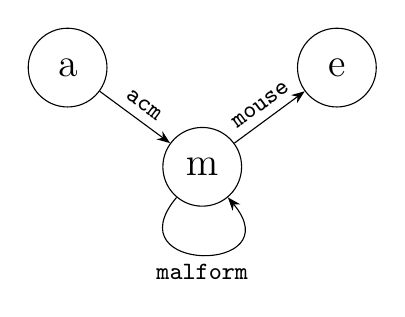
\begin{tikzpicture}[>=Stealth, scale=0.9,
  letter/.style={circle,draw,minimum size=10mm,font=\Large}]
  \node[letter] (a) at (-1.9,1.4) {a};
  \node[letter] (m) at (0,0) {m};
  \node[letter] (e) at (1.9,1.4) {e};
  \draw[->] (a) -- node[above,sloped,font=\small\ttfamily] {acm} (m);
  \draw[->] (m) to[out=230,in=310,looseness=5]
    node[below,font=\small\ttfamily] {malform} (m);
  \draw[->] (m) -- node[above,sloped,font=\small\ttfamily] {mouse} (e);
\end{tikzpicture}\\
\small Hình 5: mô hình lấy chữ cái làm đỉnh và từ làm cạnh.
\end{center}

\paragraph{Nhận xét.}
So sánh hai mô hình trên, mô hình 1 rất trực quan, còn mô hình 2 cần một chút
tư duy ngược. Ta thường quen với cách ``đỉnh biểu diễn phần tử, cạnh biểu diễn
quan hệ giữa phần tử''. Mô hình 2 làm ngược lại: phần tử nằm trên cạnh, còn
đỉnh đóng vai trò nối các phần tử với nhau. Khi giải bài, đôi khi phải cân
nhắc và cải tiến mô hình nhiều lần, thậm chí phá vỡ lối nghĩ cũ, mới tìm được
cách giải tốt.

\subsection{Ví dụ 2: Quản lý kho}

\paragraph{Mô tả bài toán.}
Một công ty có \(N\) cửa hàng, mỗi cửa hàng bán cùng \(M\) loại hàng hóa. Công
ty có một kho lớn để sắp xếp và đóng hàng trước khi chuyển tới các cửa hàng.
Một lượng hàng của một loại được đặt vào một thùng và dán nhãn loại hàng từ
\(1\) tới \(M\). Vì thế có tổng cộng \(N\times M\) thùng, và mỗi cửa hàng sẽ
nhận đúng một thùng của từng loại.

Kho nằm trong một tòa nhà hẹp nên các thùng phải xếp thành một hàng. Để tăng
tốc phân phối, người quản lý muốn sắp xếp lại hàng thùng. Một thứ tự tốt là:
\(M\) thùng đầu có nhãn khác nhau để gửi tới cửa hàng \(1\), \(M\) thùng tiếp
theo có nhãn khác nhau để gửi tới cửa hàng \(2\), và cứ thế tiếp tục. Ở trạng
thái ban đầu chỉ có một vị trí trống ở cuối hàng. Mỗi lần chỉ được chuyển một
thùng vào vị trí trống hiện tại, và sau khi kết thúc mọi thao tác, vị trí
trống phải trở lại cuối hàng. Hãy tính số lần di chuyển ít nhất và một cách di
chuyển tương ứng.

Quy mô dữ liệu: \(1\le N,M\le 400\).

\paragraph{Phân tích.}
Xây dựng đồ thị hai phía có hướng \(G\) với tập đỉnh
\[
  V=\{p_1,p_2,\ldots,p_N\}\cup\{q_1,q_2,\ldots,q_M\}.
\]
Các đỉnh \(p_1,\ldots,p_N\) biểu diễn cửa hàng, còn
\(q_1,\ldots,q_M\) biểu diễn loại hàng. Gọi \(t_{i,j}\) là số thùng nhãn
\(j\) đang nằm trong đoạn thùng dành cho cửa hàng \(i\), tức từ vị trí
\((i-1)M+1\) tới \(iM\). Mục tiêu là sau khi sắp xếp lại, mọi
\(t_{i,j}=1\).

Với mỗi cặp \(i,j\), nếu \(t_{i,j}>1\), nối \(t_{i,j}-1\) cạnh từ \(p_i\) tới
\(q_j\), biểu thị cửa hàng \(i\) đang thừa \(t_{i,j}-1\) thùng loại \(j\). Nếu
\(t_{i,j}<1\), nối \(1-t_{i,j}\) cạnh từ \(q_j\) tới \(p_i\), biểu thị cửa
hàng \(i\) đang thiếu \(1-t_{i,j}\) thùng loại \(j\).

Chẳng hạn với \(N=5,M=6\), hàng thùng ban đầu có thể là
\[
\begin{array}{c|cccccc}
\text{cửa hàng }1&4&1&3&1&6&5\\
\text{cửa hàng }2&2&3&2&3&5&6\\
\text{cửa hàng }3&2&1&4&5&6&4\\
\text{cửa hàng }4&1&3&2&4&5&5\\
\text{cửa hàng }5&1&2&3&4&6&6
\end{array}
\]
Từ bảng này ta lập đồ thị hai phía theo quy tắc trên.

\begin{center}
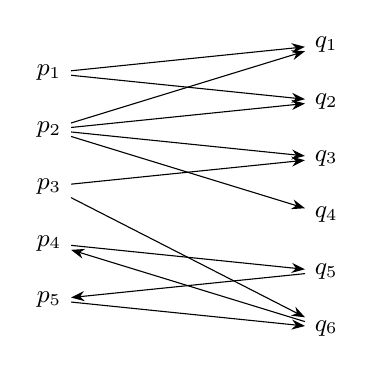
\begin{tikzpicture}[>=Stealth, x=1.1cm, y=0.72cm,
  every node/.style={font=\small}]
  \foreach \i/\name in {1/p_1,2/p_2,3/p_3,4/p_4,5/p_5} {
    \node (p\i) at (0,6-\i) {\(\name\)};
  }
  \foreach \j/\name in {1/q_1,2/q_2,3/q_3,4/q_4,5/q_5,6/q_6} {
    \node (q\j) at (3.2,6.5-\j) {\(\name\)};
  }
  \draw[->] (p1) -- (q1);
  \draw[->] (p1) -- (q2);
  \draw[->] (p2) -- (q1);
  \draw[->] (p2) -- (q2);
  \draw[->] (p2) -- (q3);
  \draw[->] (p2) -- (q4);
  \draw[->] (p3) -- (q3);
  \draw[->] (p3) -- (q6);
  \draw[->] (p4) -- (q5);
  \draw[->] (q5) -- (p5);
  \draw[->] (p5) -- (q6);
  \draw[->] (q6) -- (p4);
\end{tikzpicture}\\
\small Hình 6: đồ thị hai phía sinh từ mẫu quản lý kho.
\end{center}

Xét vị trí của ô trống trong toàn bộ quá trình sắp xếp. Ban đầu và cuối cùng,
ô trống ở cuối hàng; ngoài ra cũng có thể có một số trạng thái trung gian mà
ô trống lại ở cuối hàng. Ta gọi chuỗi các bước di chuyển giữa hai trạng thái
liên tiếp như vậy là một giai đoạn.

Một giai đoạn di chuyển tương ứng một-một với một chu trình đơn trong \(G\).
Ví dụ, chu trình
\[
  \{(p_4,q_5),(q_5,p_5),(p_5,q_6),(q_6,p_4)\}
\]
tương ứng với dãy thao tác
\[
  30\to31,\qquad 24\to30,\qquad 31\to24.
\]

Vì thế bài toán chuyển thành: tìm một số chu trình không có cạnh chung trong
\(G\) sao cho chúng phủ toàn bộ cạnh của \(G\). Một chu trình độ dài
\(2\,\mathit{tot}\) tương ứng \(\mathit{tot}+1\) lần di chuyển. Nếu dùng \(c\)
chu trình để phủ \(G\), tổng số lần di chuyển là
\[
  \mathit{sum}=\frac{|E|}{2}+c.
\]
Do cần \(\mathit{sum}\) nhỏ nhất, ta cần số chu trình \(c\) nhỏ nhất.

Trong \(G\), với mọi \(p_i\), bậc vào bằng bậc ra; với mọi \(q_j\), bậc vào
cũng bằng bậc ra. Do đó mỗi thành phần liên thông mạnh cực đại của \(G\) đều
có chu trình Euler. Hiển nhiên dùng chu trình Euler của từng thành phần liên
thông mạnh cực đại để phủ \(G\) sẽ đạt số chu trình ít nhất.

Thuật toán đầy đủ:
\begin{enumerate}
  \item Lập đồ thị hai phía có hướng \(G\).
  \item Tìm mọi thành phần liên thông mạnh cực đại của \(G\).
  \item Với mỗi thành phần liên thông mạnh cực đại, tìm một chu trình Euler.
  \item Từ các chu trình Euler đó, dựng phương án di chuyển tương ứng.
\end{enumerate}

\paragraph{Nhận xét.}
Một số bài toán thoạt nhìn không liên quan nhiều tới chu trình Euler, thậm chí
không giống bài toán đồ thị, vẫn có thể được chuyển hóa khéo léo thành bài
toán tìm chu trình Euler, qua đó giải rất hiệu quả. Điều này cho thấy tính
linh hoạt của ứng dụng chu trình Euler.

\subsection{Ví dụ 3: Bài toán người đưa thư Trung Hoa, phiên bản 1}

\paragraph{Mô tả bài toán.}
Hệ thống giao thông của thành phố \(A\) gồm các giao lộ và các con đường, mỗi
con đường nối hai giao lộ. Mọi đường đều đi được hai chiều và có một độ dài.
Một người đưa thư xuất phát từ bưu cục, cần đi qua mọi con đường thuộc khu
vực phụ trách rồi cuối cùng quay lại bưu cục; một con đường có thể đi qua hơn
một lần. Hỏi nên sắp xếp lộ trình thế nào để tổng độ dài đi được là nhỏ nhất?

\paragraph{Phân tích.}
Xem giao lộ là đỉnh, đường là cạnh vô hướng, ta được đồ thị vô hướng \(G\).
Nếu \(G\) không liên thông thì chắc chắn vô nghiệm. Nếu \(G\) là đồ thị Euler,
rõ ràng bất kỳ chu trình Euler nào của \(G\) cũng là lộ trình tối ưu.

Nếu \(G\) có đúng hai đỉnh bậc lẻ \(v_1,v_2\), thì \(G\) tồn tại một đường đi
Euler \(P\) từ \(v_1\) tới \(v_2\). Tìm thêm một đường đi ngắn nhất \(R\) từ
\(v_2\) về \(v_1\), rồi nối \(R\) sau \(P\), ta được một chu trình hoàn chỉnh.
Có thể chứng minh lộ trình này là tối ưu.

Nếu số đỉnh bậc lẻ lớn hơn \(2\), ta làm thế nào? Trong trường hợp hai đỉnh
bậc lẻ, thực chất ta đã thêm các cạnh của đường đi ngắn nhất \(R\) vào \(G\),
tạo đồ thị mới \(G'=G\cup R\); một chu trình Euler của \(G'\) chính là lộ
trình tối ưu. Thêm một đường đi bất kỳ \(R\) sẽ làm bậc hai đầu mút của \(R\)
tăng \(1\), tức đổi tính chẵn lẻ; các đỉnh bên trong \(R\) tăng bậc thêm \(2\)
nên không đổi tính chẵn lẻ. Vì vậy hai đầu mút của mỗi đường đi được thêm nên
là hai đỉnh bậc lẻ, nhờ đó mỗi lần thêm đường đi giảm được \(2\) đỉnh bậc lẻ.

Trong mọi đồ thị, số đỉnh bậc lẻ luôn là chẵn vì
\[
  \sum_{v\in V}d(v)=2|E|.
\]
Giả sử \(G\) có \(k\) đỉnh bậc lẻ. Ta luôn có thể thêm \(k/2\) đường đi để mọi
đỉnh đều có bậc chẵn.

Vấn đề còn lại là làm sao để tổng độ dài của \(k/2\) đường đi được thêm là nhỏ
nhất. Mỗi đường đi được thêm hiển nhiên phải là đường đi ngắn nhất giữa hai
đầu mút của nó. Ngoài ra, cần ghép cặp \(k\) đỉnh bậc lẻ sao cho tổng độ dài
đường đi ngắn nhất giữa các cặp là nhỏ nhất. Dựng đồ thị đầy đủ vô hướng
\(H\), trong đó tập đỉnh là \(k\) đỉnh bậc lẻ của \(G\), trọng số cạnh là độ
dài đường đi ngắn nhất giữa hai đỉnh tương ứng. Khi đó một bộ ghép hoàn hảo
trọng số nhỏ nhất của \(H\) tương ứng phương án tối ưu. Bộ ghép trọng số nhỏ
nhất trên đồ thị đầy đủ vô hướng có thể giải bằng thuật toán của Edmonds trong
thời gian đa thức. Cuối cùng, thêm cạnh vào \(G\) theo bộ ghép để được \(G'\),
rồi tìm chu trình Euler trong \(G'\).

Thuật toán đầy đủ:
\begin{enumerate}
  \item Nếu \(G\) liên thông, chuyển sang bước 2; nếu không, trả về vô nghiệm.
  \item Lấy các đỉnh bậc lẻ của \(G\) làm tập đỉnh của \(H\).
  \item Tính độ dài đường đi ngắn nhất giữa mọi cặp đỉnh bậc lẻ trong \(G\),
  dùng làm trọng số cạnh tương ứng trong \(H\).
  \item Tìm bộ ghép trọng số nhỏ nhất của \(H\).
  \item Với mỗi cạnh ghép, thêm đường đi mà cạnh đó đại diện vào \(G\), thu
  được \(G'\).
  \item Tìm chu trình Euler của \(G'\); đó là lộ trình tối ưu cần tìm.
\end{enumerate}

\subsection{Ví dụ 4: Bài toán người đưa thư Trung Hoa, phiên bản 2}

\paragraph{Mô tả bài toán.}
Hệ thống giao thông của thành phố \(A\) gồm các giao lộ và các con đường, mỗi
con đường nối hai giao lộ. Mọi đường đều chỉ đi được một chiều và có một độ
dài. Một người đưa thư xuất phát từ bưu cục, cần đi qua mọi con đường thuộc
khu vực phụ trách rồi cuối cùng quay lại bưu cục; một con đường có thể đi qua
hơn một lần. Hỏi nên sắp xếp lộ trình thế nào để tổng độ dài đi được là nhỏ
nhất?

\paragraph{Phân tích.}
Điểm khác duy nhất so với ví dụ 3 là mọi cạnh đều có hướng. Nếu đồ thị nền của
\(G\) không liên thông thì chắc chắn vô nghiệm. Ngoài ra, nếu tồn tại một đỉnh
có bậc vào hoặc bậc ra bằng \(0\), không thể có chu trình đi qua đỉnh đó; tình
huống này cũng vô nghiệm.

Tương tự ví dụ 3, ta xét việc thêm một số đường đi vào \(G\) để được đồ thị
Euler \(G'\), rồi tìm chu trình Euler trong \(G'\).

Trước hết tính với mỗi đỉnh \(v\)
\[
  d'(v)=\indeg(v)-\outdeg(v).
\]
Nếu mọi \(d'(v)=0\), \(G\) đã có chu trình Euler. Ngược lại, vì
\(\sum_{v\in V}d'(v)=0\), các giá trị \(d'(v)\) phải có cả dương và âm. Với
đỉnh \(v\) có \(d'(v)>0\), cần thêm \(d'(v)\) đường đi xuất phát từ \(v\). Với
đỉnh \(v\) có \(d'(v)<0\), cần thêm \(-d'(v)\) đường đi kết thúc tại \(v\).
Với đỉnh \(v\) có \(d'(v)=0\), \(v\) không cần là đầu mút của đường đi thêm
vào; nếu vừa có đường đi kết thúc ở \(v\) vừa có đường đi xuất phát từ \(v\),
ta có thể nối hai đường đi đó lại.

Mô hình này rất giống mạng dòng chảy: đỉnh có \(d'(v)>0\) là nguồn, phát
\(d'(v)\) đơn vị dòng; đỉnh có \(d'(v)<0\) là đích, nhận \(-d'(v)\) đơn vị
dòng; đỉnh có \(d'(v)=0\) là đỉnh trung gian, lượng vào bằng lượng ra. Bài gốc
còn yêu cầu tổng độ dài đường đi thêm vào nhỏ nhất, vì vậy đặt chi phí
\(w(e)\) của mỗi cạnh trong mạng bằng độ dài cạnh tương ứng trong \(G\). Khi
đó tìm dòng cực đại chi phí nhỏ nhất trong mạng sẽ tối thiểu hóa
\[
  \sum_{e\in E} f(e)w(e).
\]

Cụ thể, dựng mạng \(N\) như sau:
\begin{enumerate}
  \item Tập đỉnh gồm mọi đỉnh của \(G\), thêm siêu nguồn \(s\) và siêu đích
  \(t\).
  \item Với mỗi cạnh \((u,v)\) của \(G\), thêm cạnh \((u,v)\) trong \(N\), dung
  lượng \(\infty\), chi phí bằng độ dài cạnh.
  \item Từ \(s\) tới mọi đỉnh \(v\) có \(d'(v)>0\), thêm cạnh \((s,v)\), dung
  lượng \(d'(v)\), chi phí \(0\).
  \item Từ mọi đỉnh \(u\) có \(d'(u)<0\) tới \(t\), thêm cạnh \((u,t)\), dung
  lượng \(-d'(u)\), chi phí \(0\).
\end{enumerate}

Thuật toán đầy đủ:
\begin{enumerate}
  \item Nếu đồ thị nền của \(G\) liên thông và mọi đỉnh có bậc vào, bậc ra đều
  khác \(0\), chuyển sang bước 2; nếu không, trả về vô nghiệm.
  \item Tính \(d'(v)\) cho mọi đỉnh \(v\).
  \item Dựng mạng \(N\).
  \item Tìm dòng cực đại chi phí nhỏ nhất trong \(N\).
  \item Với mỗi cạnh \((u,v)\) của \(N\) có dòng \(f(u,v)\), thêm cạnh
  \((u,v)\) vào \(G\) đúng \(f(u,v)\) lần, thu được \(G'\).
  \item Tìm chu trình Euler của \(G'\); đó là lộ trình tối ưu.
\end{enumerate}

\paragraph{Mở rộng.}
Nếu thay điều kiện thành: một số đường đi được hai chiều, một số đường chỉ đi
được một chiều, thì bài toán trở nên khó hơn; biến thể này đã được chứng minh
là NP-đầy đủ.

\paragraph{Nhận xét.}
Ví dụ 3, ví dụ 4 và biến thể mở rộng chỉ khác nhau vài chữ trong điều kiện,
nhưng lời giải khác hẳn nhau. Điều đó nhắc ta phải đọc đề thật kỹ và suy nghĩ
sát các điều kiện then chốt. Đồng thời, trong quá trình luyện tập nên thường
xuyên tự hỏi: nếu thay một điều kiện thì bài toán sẽ ra sao? Suy nghĩ và giải
một chuỗi bài toán có nhiều điểm giống nhau như vậy sẽ rèn được chiều sâu tư
duy.

\subsection{Ví dụ 5: Máy đánh bạc}

\paragraph{Mô tả bài toán.}
Một máy đánh bạc gồm \(n\) bộ sinh số nguyên \(T_1,T_2,\ldots,T_n\). Bộ sinh
\(T_i\) chỉ có thể sinh các số trong tập \(S_i\), với \(S_i\subseteq
\{1,2,\ldots,n\}\). Tập \(S_i\) có thể rỗng. Ở mọi thời điểm khi máy chạy,
đúng một bộ sinh đang hoạt động. Ban đầu chỉ có \(T_1\) hoạt động. Nếu bộ sinh
đang hoạt động là \(T_i\) và \(S_i\ne\varnothing\), người chơi chọn một số
\(r\in S_i\); máy xóa \(r\) khỏi \(S_i\) và chuyển trạng thái hoạt động sang
\(T_r\). Nếu \(S_i=\varnothing\), trò chơi kết thúc. Nếu bộ sinh hoạt động
cuối cùng là \(T_1\), đồng thời khi trò chơi kết thúc mọi \(S_i\) đều rỗng,
người chơi thua; ngược lại người chơi thắng.

Trước khi chơi, cần viết chương trình phán đoán có thể thắng hay không. Nếu
có, chương trình phải đưa ra cách chọn số phù hợp ở từng bước.

Quy mô dữ liệu:
\[
  1\le n\le 1000,\qquad \sum_{i=1}^n |S_i|\le 12000.
\]

\paragraph{Phân tích.}
Ta trừu tượng hóa bài toán thành đồ thị. Dựng đồ thị có hướng \(G\) với tập
đỉnh \(V=\{v_1,v_2,\ldots,v_n\}\), biểu diễn \(n\) bộ sinh. Nếu \(T_i\) có thể
sinh \(j\), nối một cạnh có hướng từ \(v_i\) tới \(v_j\). Trong bài này, mỗi
quá trình chơi tương ứng một đường đi đơn bắt đầu từ \(v_1\). Đặc biệt, một
quá trình thua tương ứng một chu trình Euler bắt đầu từ \(v_1\).

Nếu người chơi dù chọn thế nào cũng thua, đồ thị \(G\) có tính chất sau: xuất
phát từ \(v_1\), miễn là không cố ý đi lại một cạnh đã đi, cuối cùng chắc chắn
đi được một chu trình Euler và không bị kẹt giữa đường. Ta gọi loại đồ thị này
là đồ thị Euler ngẫu nhiên. Rõ ràng đồ thị Euler ngẫu nhiên phải là đồ thị
Euler. Theo các kết luận về đồ thị Euler, nếu đồ thị nền không liên thông hoặc
nếu có đỉnh \(v_i\) mà bậc vào khác bậc ra, người chơi chắc chắn không rơi vào
tình huống thua với mọi lựa chọn. Vì vậy phần sau chỉ xét trường hợp \(G\) là
đồ thị Euler.

Ta có một nhận xét quan trọng: với bất kỳ quá trình chơi nào, bộ sinh hoạt
động cuối cùng chắc chắn là \(T_1\). Nếu bộ sinh cuối cùng là \(T_i\) với
\(1<i\le n\), thì trong đường đi tương ứng, số lần đi vào \(v_i\) lớn hơn số
lần rời khỏi \(v_i\) đúng \(1\). Nhưng vì bậc vào của \(v_i\) bằng bậc ra, lúc
đó vẫn phải còn một cạnh xuất phát từ \(v_i\) chưa được dùng, trái với điều
kiện trò chơi đã kết thúc. Nói cách khác, mọi quá trình chơi đều tương ứng một
chu trình đơn.

Giả sử một quá trình chơi tương ứng chu trình \(C\) trong \(G\). Xóa các cạnh
của \(C\) khỏi \(G\), thu được đồ thị còn lại \(G'=G-C\). Khi đó mọi đỉnh của
\(G'\) vẫn có bậc vào bằng bậc ra. Có hai trường hợp. Nếu \(G'\) không còn
cạnh, đây là một quá trình thua. Ngược lại, mỗi thành phần liên thông mạnh cực
đại của \(G'\) đều có chu trình Euler. Chú ý rằng \(v_1\) chắc chắn là đỉnh cô
lập trong \(G'\), nếu không trò chơi chưa thể kết thúc. Do đó trong \(G'\)
chắc chắn tồn tại một chu trình không đi qua \(v_1\).

Kết luận: người chơi có thể thắng khi và chỉ khi \(G\) có một đồ thị con
\(G'\) gồm các chu trình không đi qua \(v_1\), và quá trình thắng tương ứng
chu trình Euler trong đồ thị bù cạnh \(G_0=G-G'\).

Còn phải tìm một chu trình trong \(G\) không đi qua \(v_1\). Chỉ cần xóa đỉnh
\(v_1\) khỏi \(G\), rồi duyệt sâu trên phần còn lại. Nếu trong quá trình DFS,
phát hiện một đỉnh \(v\) có cạnh ngược tới tổ tiên \(u\), thì đường trên cây
DFS từ \(u\) tới \(v\) cộng với cạnh \((v,u)\) tạo thành một chu trình.

Thuật toán đầy đủ:
\begin{enumerate}
  \item Dựng đồ thị có hướng \(G\).
  \item Kiểm tra \(G\) có chu trình Euler hay không. Nếu không, sinh tùy ý một
  quá trình chơi không thua, trả về và kết thúc.
  \item Kiểm tra \(G\) có chu trình \(C\) không đi qua \(v_1\) hay không. Nếu
  có, đặt \(G_0=G-C\), trả về chu trình Euler trong \(G_0\) và kết thúc.
  \item Nếu không có chu trình như vậy, kết luận trò chơi chắc chắn thua.
\end{enumerate}

\section{Tổng kết}

Chu trình Euler là chu trình đi qua mọi cạnh của đồ thị đúng một lần. Mô hình
chu trình Euler ngắn gọn, linh hoạt, dễ cài đặt và có thuật toán hiệu quả, nên
được ứng dụng rộng rãi. Trong bài toán thực tế, nếu có thể tập trung thông tin
chính lên các cạnh và chuyển yêu cầu thành việc đi qua mọi cạnh của đồ thị,
ta có thể vận dụng tốt các tính chất và thuật toán của chu trình Euler để giải
bài hiệu quả. Vì vậy, lập mô hình đóng vai trò then chốt trong quá trình giải
bài. Mô hình của bài toán thường không hiện rõ ngay từ đầu; ta phải phân tích
kỹ, nghiên cứu bản chất vấn đề, mở rộng hướng suy nghĩ và thử cách nhìn mới
để xây dựng được mô hình phù hợp.

\section*{Lời cảm ơn}

Trong quá trình viết bài, tác giả nhận được sự hướng dẫn tận tình của cô Li
Shuping tại Trung học trực thuộc Đại học Sư phạm Hồ Nam. Tác giả xin chân
thành cảm ơn cô, đồng thời cảm ơn các bạn trong nhóm tin học của lớp và các
bạn trong đội tuyển tập huấn đã giúp đỡ, ủng hộ.

\begin{thebibliography}{9}
\bibitem{liu-huang}
Liu Rujia, Huang Liang. \textit{Nghệ thuật thuật toán và thi tin học}.
\bibitem{lu-lu}
Lu Kaicheng, Lu Huaming. \textit{Lý thuyết đồ thị và ứng dụng}.
\bibitem{dai-hu-chen}
Dai Yiqi, Hu Guanzhang, Chen Wei. \textit{Lý thuyết đồ thị và cấu trúc đại số}.
\bibitem{edmonds-johnson}
J. Edmonds, E. Johnson. \textit{Matching, Euler tours, and the Chinese postman}.
\bibitem{papadimitriou}
C. Papadimitriou. \textit{The complexity of edge traversing}.
\bibitem{boi2001}
Baltic Olympiad in Informatics 2001, lời giải chính thức.
\end{thebibliography}

\appendix

\section{Cài đặt tham khảo cho chu trình Euler vô hướng}

Hai chương trình Pascal trong tài liệu gốc lần lượt cài thuật toán đệ quy và
không đệ quy cho đồ thị vô hướng. Dưới đây là mã giả giữ lại cấu trúc chính:
kiểm tra liên thông sau khi bỏ đỉnh cô lập, kiểm tra mọi bậc là chẵn, rồi dùng
Hierholzer để sinh chu trình.

\begin{verbatim}
function has_euler_circuit(G)
    remove all isolated vertices from the connectivity test
    if remaining graph is not connected then return false
    for each vertex v do
        if degree(v) is odd then return false
    return true
end function

procedure recursive_hierholzer(u)
    while u has an unused incident edge e = (u, v) do
        mark e and its reverse as used
        recursive_hierholzer(v)
        append e to answer
    end while
end procedure
\end{verbatim}

Phiên bản không đệ quy có thể viết bằng một ngăn xếp đỉnh và một danh sách
cạnh kết quả:
\begin{verbatim}
procedure iterative_hierholzer(start)
    stack <- [start]
    answer <- empty list
    while stack is not empty do
        u <- top(stack)
        if u has an unused incident edge (u, v) then
            mark (u, v) and (v, u) as used
            push v into stack
        else
            pop u from stack
            if stack is not empty then
                append edge(top(stack), u) to answer
            end if
        end if
    end while
    reverse answer
end procedure
\end{verbatim}

\section{Nguyên đề tiếng Anh của ví dụ 1: Play on Words}

Một số cánh cửa bí mật chứa một câu đố chữ rất thú vị. Đội khảo cổ phải giải
câu đố ấy để mở cửa; vì không còn cách nào khác để mở các cánh cửa này, câu đố
rất quan trọng với họ.

Trên mỗi cánh cửa có rất nhiều tấm bảng nam châm. Mỗi tấm bảng có một từ viết
trên đó. Các tấm bảng phải được sắp thành một dãy sao cho mỗi từ bắt đầu bằng
cùng chữ cái với chữ cuối của từ đứng trước nó. Ví dụ, từ \texttt{acm} có thể
được theo sau bởi từ \texttt{Motorola}. Nhiệm vụ là viết chương trình đọc danh
sách từ và xác định liệu có thể sắp xếp tất cả tấm bảng thành một dãy theo quy
tắc trên, từ đó mở được cánh cửa hay không.

\paragraph{Input Specification.}
Dữ liệu vào gồm \(T\) bộ kiểm thử; số \(T\) nằm ở dòng đầu của tệp vào. Mỗi bộ
bắt đầu bằng một dòng chứa số nguyên \(N\), số tấm bảng, với
\[
  1\le N\le 100000.
\]
Sau đó có đúng \(N\) dòng, mỗi dòng chứa một từ. Mỗi từ có ít nhất 2 và nhiều
nhất 1000 chữ cái thường, nghĩa là chỉ gồm các chữ cái từ \texttt{a} đến
\texttt{z}. Một từ có thể xuất hiện nhiều lần trong danh sách.

\paragraph{Output Specification.}
Chương trình phải xác định liệu có thể sắp xếp mọi tấm bảng thành một dãy sao
cho chữ đầu của mỗi từ bằng chữ cuối của từ đứng trước nó hay không. Tất cả tấm
bảng trong danh sách phải được dùng, mỗi tấm đúng một lần. Nếu một từ xuất hiện
nhiều lần thì phải dùng đúng số lần ấy.

Nếu tồn tại một thứ tự như vậy, in câu:
\begin{verbatim}
Ordering is possible.
\end{verbatim}
Ngược lại, in:
\begin{verbatim}
The door cannot be opened.
\end{verbatim}

\begin{verbatim}
Sample Input
3
2
acm
ibm
3
acm
malform
mouse
2
ok
ok

Output for the Sample Input
The door cannot be opened.
Ordering is possible.
The door cannot be opened.
\end{verbatim}

\section{Nguyên đề tiếng Anh của ví dụ 2: Depot Rearrangement}

Một công ty vận hành \(N\) cửa hàng, mỗi cửa hàng bán \(M\) sản phẩm khác nhau.
Công ty có một kho lớn để đóng gói sản phẩm trước khi giao đến các cửa hàng.
Mỗi cửa hàng nhận cùng số lượng mặt hàng của từng loại sản phẩm. Vì vậy công ty
đóng một số mặt hàng của một loại sản phẩm vào một thùng và dán nhãn thùng bằng
mã sản phẩm; các sản phẩm được đánh số từ 1 đến \(M\). Sau khi đóng gói, trong
kho có \(N\cdot M\) thùng, và với mỗi nhãn sản phẩm có đúng \(N\) thùng mang
nhãn đó.

Vì kho nằm trong một tòa nhà hẹp, các thùng được xếp thành một hàng. Để tăng
tốc phân phối, người quản lý kho muốn sắp xếp lại các thùng. Do việc giao hàng
được thực hiện bằng cách gửi đúng một xe tải tới mỗi cửa hàng, và mỗi xe chở
một thùng của mỗi loại sản phẩm, một cách xếp phù hợp là: \(M\) thùng đầu tiên
trong hàng phải có nhãn khác nhau, \(M\) thùng tiếp theo cũng phải có nhãn khác
nhau, và cứ tiếp tục như vậy. Không may, chỉ có một vị trí trống ở cuối hàng để
chứa tạm một thùng. Do đó việc sắp xếp lại phải được thực hiện bằng cách liên
tiếp nhấc một thùng và chuyển nó tới vị trí trống. Sau khi sắp xếp xong, vị trí
trống phải nằm ở cuối hàng.

Mục tiêu là đạt được cách xếp yêu cầu với số lần di chuyển nhỏ nhất.

\paragraph{Task.}
Hãy viết chương trình tính một cách sắp xếp lại cần số lần di chuyển nhỏ nhất.

\paragraph{Input.}
Dòng đầu của tệp \texttt{depot.in} chứa hai số nguyên \(N,M\). \(N\) là số cửa
hàng và \(M\) là số loại sản phẩm, với
\[
  1\le N\le 400,\qquad 1\le M\le 400.
\]
Dòng thứ hai chứa \(N\cdot M\) số nguyên, là nhãn các thùng theo thứ tự ban đầu.
Mỗi mã sản phẩm \(x\), \(1\le x\le M\), xuất hiện đúng \(N\) lần trên dòng này.

\paragraph{Output.}
Dòng đầu của tệp \texttt{depot.out} chứa một số nguyên \(S\), số lần di chuyển
tối thiểu cần thiết để thu được một thứ tự hợp lệ của hàng thùng (subtask A).
\(S\) dòng tiếp theo mô tả một cách sắp xếp lại (subtask B). Mỗi dòng chứa một
cặp số nguyên \(x,y\), nghĩa là chuyển thùng tại vị trí \(x\) tới vị trí \(y\).
Các vị trí được đánh số từ 1 đến \(N\cdot M+1\); ban đầu vị trí \(N\cdot M+1\)
là vị trí trống. Một thao tác từ \(x\) tới \(y\) chỉ hợp lệ nếu trước thao tác,
vị trí \(y\) đang trống. Sau thao tác, vị trí \(x\) trở thành vị trí trống. Nếu
chỉ giải subtask A thì chỉ cần in dòng đầu.

Nếu có nhiều phương án, chương trình chỉ cần in một phương án bất kỳ.

\begin{verbatim}
Example
depot.in
5 6
4 1 3 1 6 5 2 3 2 3 5 6 2 1 4 5 6 4 1 3 2 4 5 5 1 2 3 4 6 6

depot.out
8
9 31
18 9
10 18
4 10
31 4
30 31
24 30
31 24
\end{verbatim}

\section{Nguyên đề tiếng Anh của ví dụ 5: Gambling}

Một máy đánh bạc gồm \(n\) bộ sinh số nguyên \(G_1,\ldots,G_n\), với
\(1\le n\le 1000\). Bộ sinh \(G_i\) chỉ có thể sinh các số nguyên trong một tập
nhất định \(S_i\subseteq\{1,\ldots,n\}\), hoặc sinh 0, nghĩa là trò chơi kết
thúc. Tập \(S_i\) có thể rỗng. Gọi \(k_i\) là số phần tử của \(S_i\). Tổng các
giá trị \(k_i\), với \(i=1,\ldots,n\), không vượt quá 12000.

Khi \(G_i\) được kích hoạt lần đầu, nó sinh một số nguyên trong tập \(S_i\). Các
lần kích hoạt tiếp theo sẽ sinh một số trong \(S_i\) chưa từng được chọn trước
đó. Nếu không còn số nào như vậy, \(G_i\) sinh 0.

Máy bắt đầu bằng cách kích hoạt \(G_1\). Sau đó các bộ sinh được kích hoạt theo
quy tắc:
\begin{itemize}
  \item nếu một bộ sinh sinh ra số dương \(r\), bộ sinh tiếp theo được kích hoạt
  là \(G_r\);
  \item nếu sinh ra 0, máy dừng lại.
\end{itemize}

Máy thua nếu bộ sinh \(G_n\) sinh 0 và tất cả các bộ sinh còn lại đã dùng hết
tập số nguyên của chúng.

Máy được cấu tạo tốt nếu nó có thể sinh một dãy số nguyên kết thúc bằng 0 nhưng
không dẫn tới thua, tức một dãy ngắn hơn
\[
  1+\sum_{i=1}^{n} k_i.
\]

\paragraph{Task.}
Hãy viết chương trình:
\begin{itemize}
  \item đọc từ tệp \texttt{HAZ.IN} mô tả của máy, gồm số bộ sinh \(n\), các số
  \(k_i\) và các tập \(S_i\);
  \item kiểm tra máy trong tệp vào có được cấu tạo tốt hay không;
  \item nếu có, ghi một dãy số nguyên mà máy có thể sinh ra, kết thúc bằng 0 và
  không dẫn tới thua;
  \item nếu không, ghi một từ \texttt{NIE} (``không'' trong tiếng Ba Lan) vào
  tệp \texttt{HAZ.OUT}.
\end{itemize}

\paragraph{Input.}
Dòng đầu của tệp \texttt{HAZ.IN} chứa một số nguyên dương \(n\le 1000\), là số
bộ sinh. Dòng thứ \(i+1\), với \(i=1,\ldots,n\), chứa số nguyên \(k_i\), theo
sau là mọi phần tử của tập \(S_i\) theo thứ tự bất kỳ. Các số trên mỗi dòng được
phân tách bằng một dấu cách.

\paragraph{Output.}
Trong tệp \texttt{HAZ.OUT}, in một từ \texttt{NIE} nếu máy không được cấu tạo
tốt; nếu không, in một dòng chứa một dãy hữu hạn các số nguyên phù hợp, cách
nhau bởi dấu cách.

\begin{verbatim}
Example
For the input file HAZ.IN:
2
2 1 2
1 2

the correct answer is the output file HAZ.OUT:
2 2 0

For the input file HAZ.IN:
2
1 2
0

the correct answer is the output file HAZ.OUT:
NIE
\end{verbatim}

\end{document}
